\section{Business Cases}

Di seguito sono i business case individuati a partire dalla definizione dei requisiti e dall'analisi del contesto:
\begin{itemize}
	\item Procedura di registrazione di un utente (figura \ref{fig:business_case_registration}).
	\item Procedura di autenticazione di un utente registrato (figura \ref{fig:business_case_authentication}).
	\item Procedura generica per effettuare un'operazione all'interno del sistema di Home Banking (figura \ref{fig:business_case_generic_operation}).
	\item Procedura generica di controllo da parte di un'entit\`a preposta (figura \ref{fig:business_case_control_activity}).
\end{itemize}
Nei business case utilizziamo la freccia tratteggiata (\emph{message flow}) fra gateway di \emph{pool} differenti per rappresentare sinteticamente il propagarsi dell'effetto di una decisione dalla coda alla testa della freccia.
Ad esempio, nella figura \ref{fig:business_case_authentication}, la validit\`a delle credenziali viene stabilita dal software di Home Banking, e la conclusione di questa decisione si ``riflette'' nel browser del cliente, che riceve una pagina di errore o una schermata di successo a seconda del risultato.

\begin{figure*}[hbt]
	\centering
	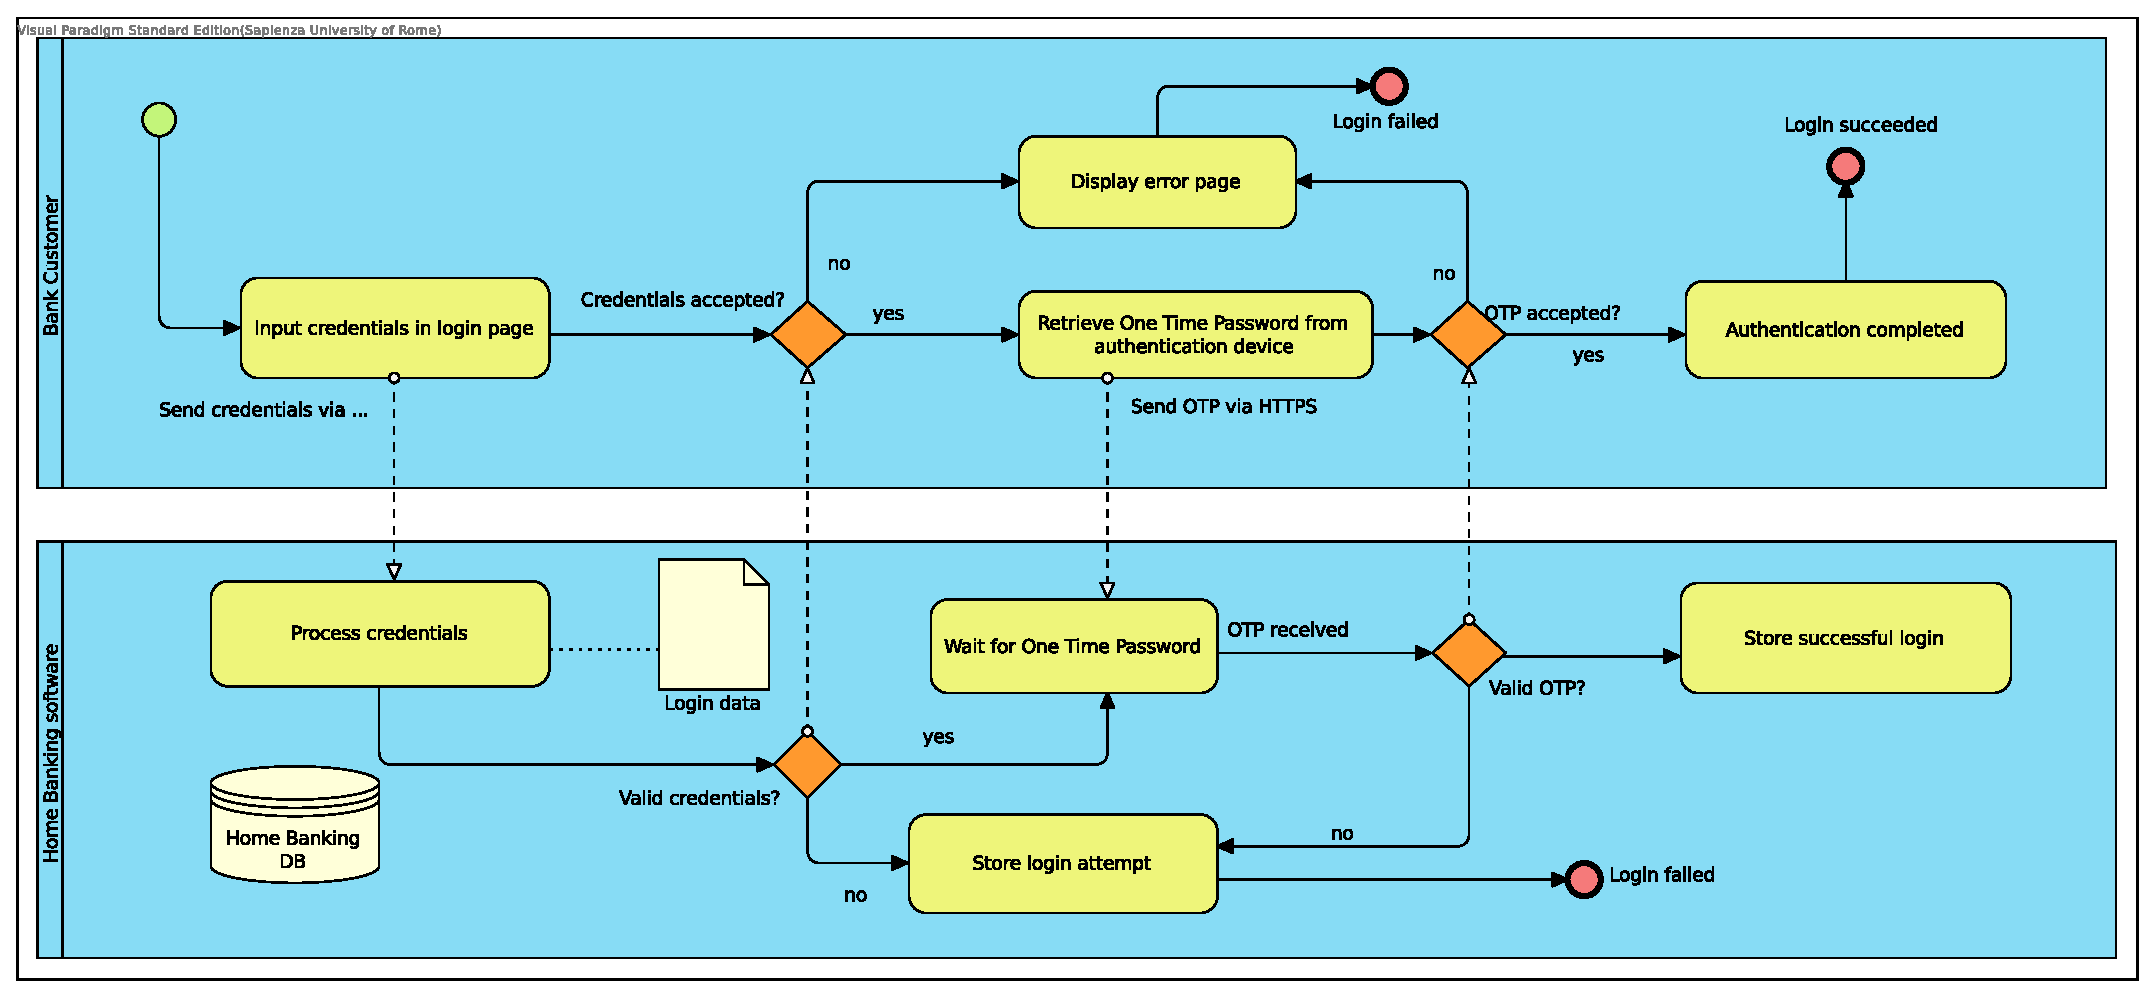
\includegraphics[width=\textheight, angle=90]{Images/Authentication.eps}
	\caption{Business case: procedura di autenticazione.}
	\label{fig:business_case_authentication}
\end{figure*}

\begin{figure*}[hbt]
	\centering
	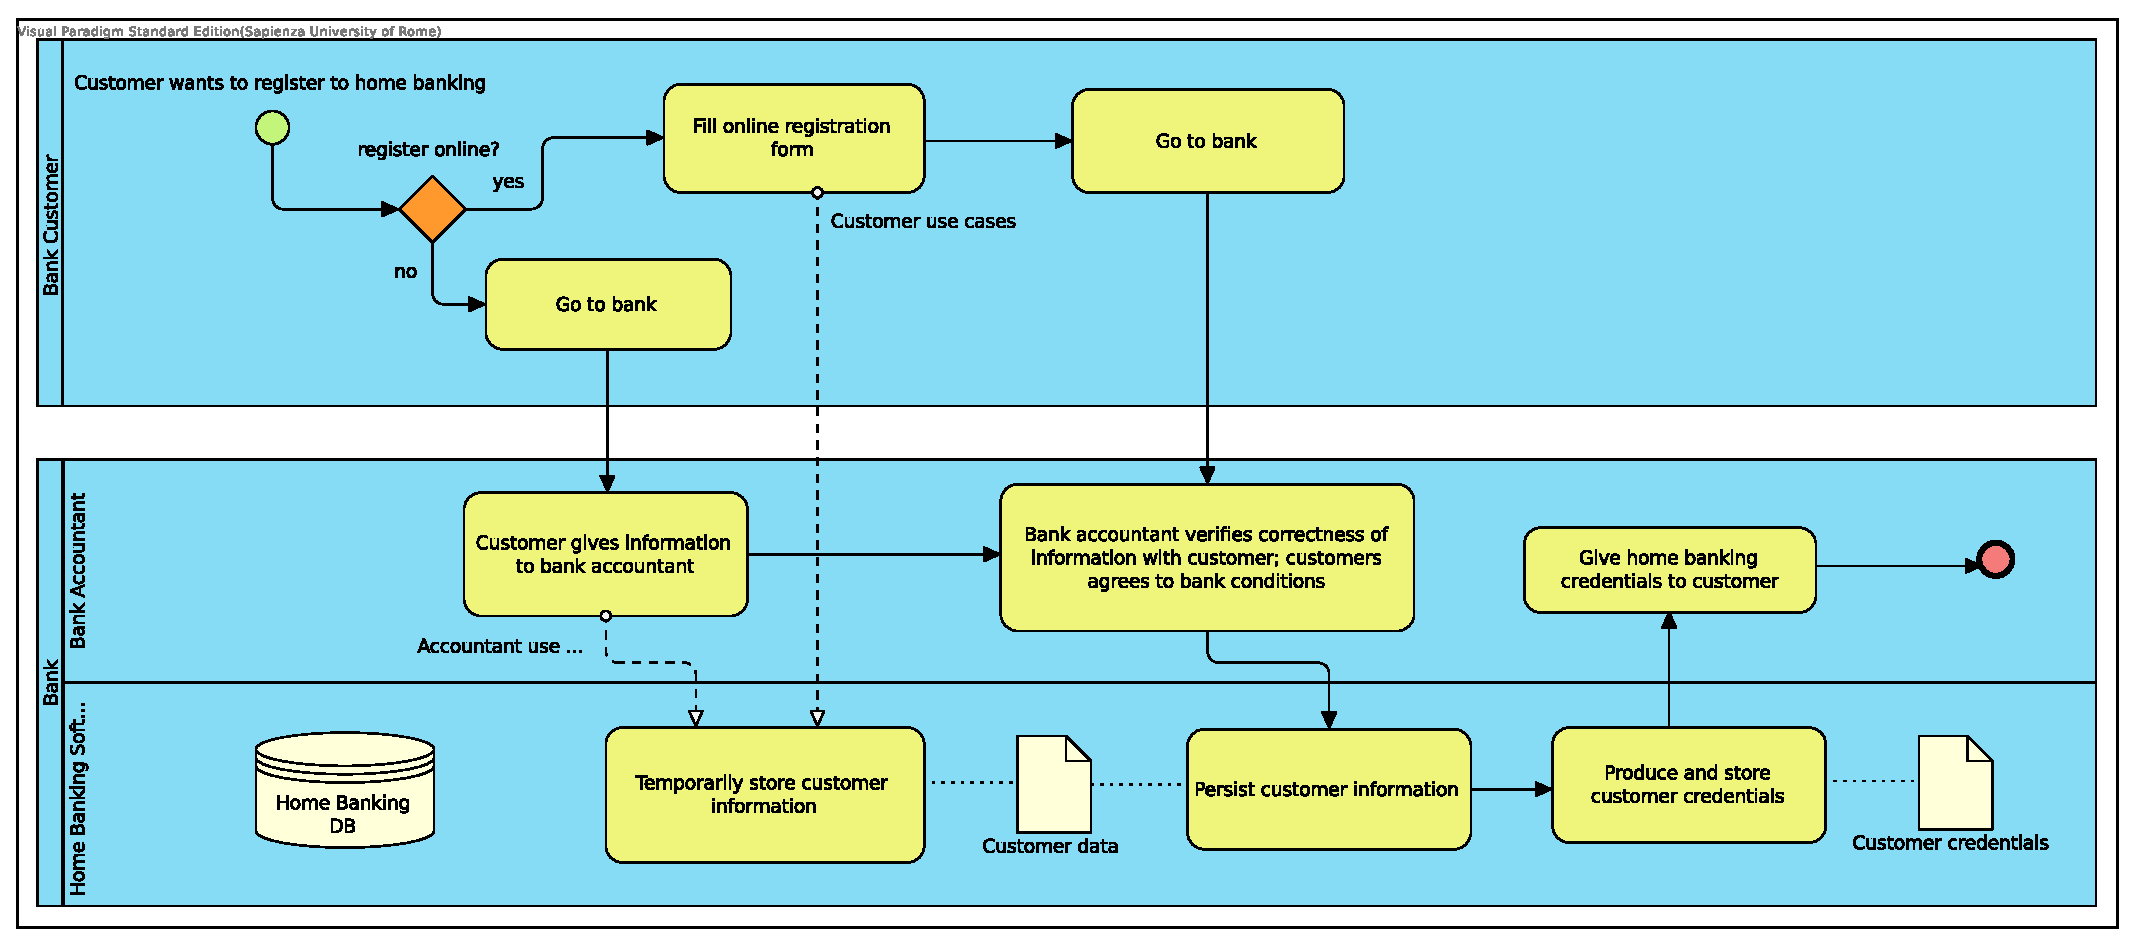
\includegraphics[width=\textheight, angle=90]{Images/Home_Banking_registration.eps}
	\caption{Business case: procedura di registrazione.}
	\label{fig:business_case_registration}
\end{figure*}

\begin{figure*}[hbt]
	\centering
	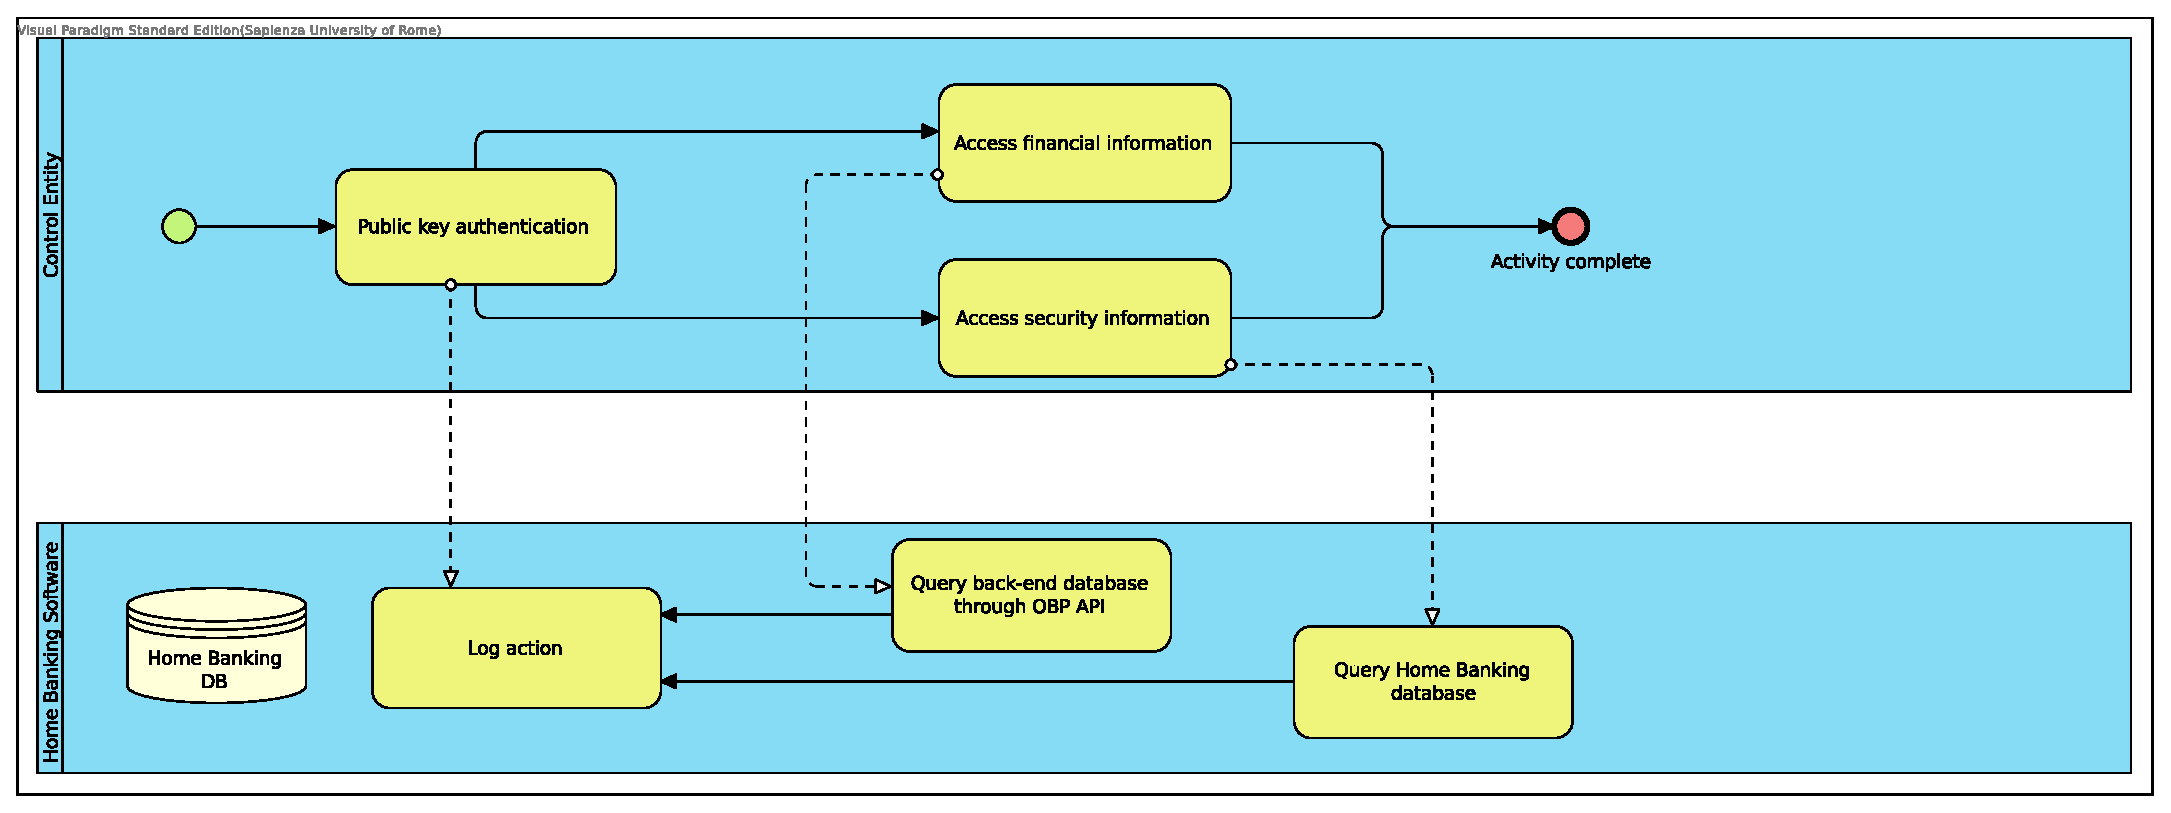
\includegraphics[width=\textheight, angle=90]{Images/Home_Banking_control_activity.eps}
	\caption{Business case: attivit\`a di controllo effettuata da enti responsabili.}
	\label{fig:business_case_control_activity}
\end{figure*}

\begin{figure*}[hbt]
	\centering
	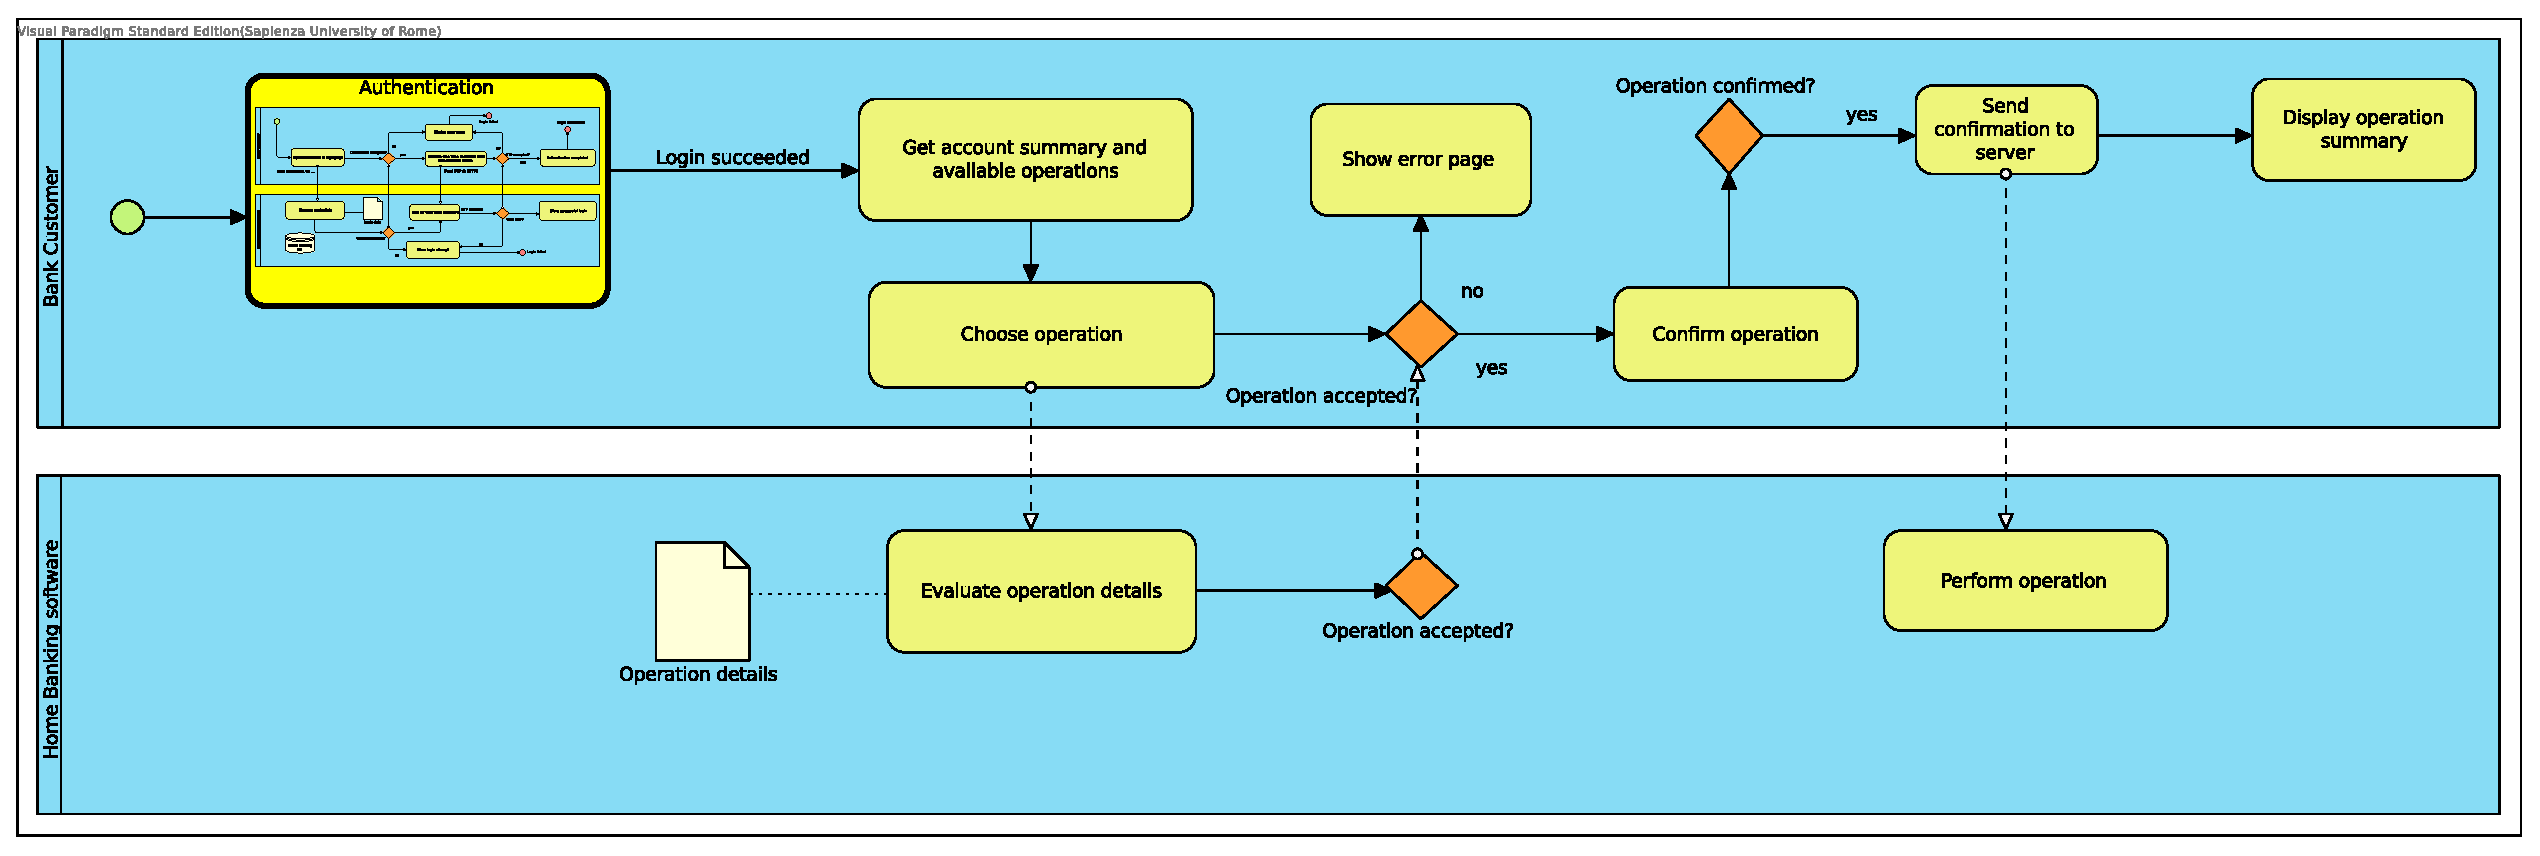
\includegraphics[width=\textheight, angle=90]{Images/Home_Banking_generic_action.eps}
	\caption{Business case: generica procedura di Home Banking effettuata da un utente del sistema.}
	\label{fig:business_case_generic_operation}
\end{figure*}